% Complete Section 4.3, original PDF 47-49 / printed 37-39.
% block: l2-de-rham-heading page:47 type:section
\section{{Example: $L^2$ de Rham 复形}}\label{sec:l2-de-rham-complex}

% block: l2-de-rham-base-domain page:47 type:ordinary-paragraph
{Hilbert 复形的典型例子是与 Riemannian 流形相伴的 de Rham 复形. 继续讨论 $\mathbb R^3$ 中区域 $\Omega$ 的情形, 并假设其具有 Lipschitz 边界. 基 Hilbert 空间取为 $W^0=W^3=L^2(\Omega)$, $W^1=W^2=L^2(\Omega;\mathbb R^3)$. 算子是 Section~\ref{sec:vector-operators-adjoints} 中讨论的那些算子: $d^0=\operatorname{grad}$, $d^1=\operatorname{curl}$, $d^2=\operatorname{div}$, 定义域分别取为 $H^1$, $H(\operatorname{curl})$ 和 $H(\operatorname{div})$. 那里已看到这些算子是闭的, 因而满足 Hilbert 复形的条件. 由空间 $V^k$ 组成的定义域复形为}
\begin{equation}\label{eq:l2-de-rham-domain-complex}
0\to H^1\xrightarrow{\operatorname{grad}}H(\operatorname{curl})\xrightarrow{\operatorname{curl}}H(\operatorname{div})\xrightarrow{\operatorname{div}}L^2\to0.
\end{equation}

% block: l2-dual-domain-complex page:47 type:ordinary-paragraph
{根据 Section~\ref{sec:vector-operators-adjoints} 中计算的伴随, 对偶复形的定义域复形 (由 $V_k^*$ 组成) 为}
\begin{equation}\label{eq:l2-dual-domain-complex}
0\leftarrow L^2\xleftarrow{-\operatorname{div}}\mathring H(\operatorname{div})\xleftarrow{\operatorname{curl}}\mathring H(\operatorname{curl})\xleftarrow{-\operatorname{grad}}\mathring H^1\leftarrow0.
\end{equation}

% block: de-rham-compactness page:48 type:ordinary-paragraph
{一个重要事实是, $L^2$ de Rham 复形满足紧性性质, 即 $V^k\cap V_k^*$ 紧嵌入 $W^k$. 对 $k=0$, 有 $V^0\cap V_0^*=H^1\cap L^2=H^1$, 由 Rellich 定理, 它在 $W^0=L^2$ 中确实是紧的. $k=3$ 的结论类似. 对 $k=1$ 和 $2$, 所需结论是 $H(\operatorname{curl})\cap\mathring H(\operatorname{div})$ 与 $\mathring H(\operatorname{curl})\cap H(\operatorname{div})$ 在 $L^2(\Omega;\mathbb R^3)$ 中紧. Picard \BookCite{62} 在具有 Lipschitz 边界的 Riemannian 流形这一更一般背景下证明了此结论. 根据 Theorem~\ref{thm:compactness-implies-fredholm}, 紧性性质意味着 de Rham 复形是 Fredholm 的: 各算子的像空间是闭的, 且调和形式空间为有限维. 特别地, 我们已证明 $\operatorname{curl}H(\operatorname{curl})$ 是闭的, 正如 Chapter~\ref{chap:unbounded-operators} 末尾所述. 下面计算调和形式空间, 并给出每个次数上的 Hodge 分解.}

% block: harmonic-zero-forms page:48 type:ordinary-paragraph
{调和 $0$-形式的空间与梯度的零空间 $\mathcal Z^0$ 相同. 这是常数空间, 或者若允许区域有多个连通分支, 则是局部常数空间. 其维数是 $\Omega$ 的连通分支数 $b_0$ (即区域的第零个 Betti 数). 由于空间 $\mathcal B^0=0$, Hodge 分解将 $L^2$ 表示为 $\operatorname{div}\mathring H(\operatorname{div})$ 与常数 (或局部常数) 函数之和.}

% block: harmonic-one-forms pages:48,49 type:ordinary-paragraph
{调和 $1$-形式的空间更复杂. 它由满足 $\operatorname{curl}p=0$, $\operatorname{div}p=0$, 且法向迹 $\gamma_n p$ 在 $\partial\Omega$ 上为零的 $L^2$ 向量场 $p$ 组成. Figure~\ref{fig:de-rham-harmonic-fields} 左图给出了这种函数的一个初等例子, 其区域是环形柱体. 在柱坐标中, 该区域由 $a\leq r\leq b$, $c\leq z\leq d$ 给出, 其中 $0<a<b$, $c<d$, 而调和形式就是 $p=\operatorname{grad}\theta$ 的倍数. 在一般区域上, $\dim\mathsf H^1=b_1$, 即第一个 Betti 数, 它在 Section~\ref{sec:simplicial-chain-complex} 中已定义, 计数贯通区域的隧道数. 对单连通区域, $b_1=0$, Hodge 分解就是经典的 Helmholtz 分解, 将向量场分解为一个梯度 (无旋的, 即旋度为零) 和一个旋度 (螺线的, 即散度为零). 对一般区域, 还必须包含调和部分:}
\[
L^2(\Omega;\mathbb R^3)=\operatorname{grad}H^1(\Omega)\BookOrthSum\operatorname{curl}\mathring H(\operatorname{curl};\Omega)\BookOrthSum\mathsf H^1.
\]

% block: de-rham-harmonic-fields-figure page:48 type:figure
\begin{figure}[htbp]\centering
\includegraphics[page=48,trim=89bp 83bp 57bp 445bp,clip,width=.85\linewidth]{../input/source/Finite Element Exterior Calculus.pdf}
\caption{{左: $\mathbb R^3$ 中环形柱体上的调和 $1$-形式. 右: 球壳上的调和 $2$-形式 (为便于观察, 已切去半个球壳).}}\label{fig:de-rham-harmonic-fields}
\end{figure}

% block: harmonic-two-forms page:49 type:ordinary-paragraph
{调和 $2$-形式的空间同样由无旋且无散的向量场组成, 但此时它们在边界上的切向迹为零. 一个初等例子是在闭球壳 $a<r<b$ 上, 用球坐标给出的 $p=\operatorname{grad}(1/r)$. 见 Figure~\ref{fig:de-rham-harmonic-fields}. 在一般区域上, $\dim\mathsf H^2=b_2$, 即区域中的空腔数. Hodge 分解仍然分解为梯度和旋度, 但边界条件不同, 调和形式空间也不同:}
\[
L^2(\Omega;\mathbb R^3)=\operatorname{grad}\mathring H^1(\Omega)\BookOrthSum\operatorname{curl}H(\operatorname{curl};\Omega)\BookOrthSum\mathsf H^2.
\]

% block: harmonic-three-forms page:49 type:ordinary-paragraph
{最后, 调和 $3$-形式的空间很简单: $\mathsf H^3=0$, 因为 $\mathring H^1$ 中没有梯度为零的非零函数. 当然, $\mathcal B_3^*$ 也为零, 因此 Hodge 分解是平凡的.}
